
%% CLASS MANUAL FOUND IN http://blog.poormansmath.net/latex-class-for-lecture-notes/ %%
%% CLASS AUTHOR Stefano Maggiolo %%

%%%%%%%%%%%%%%%  TITLE PAGE  %%%%%%%%%%%%%%%%%%%
\documentclass[english,course]{Notes}
\title{OOSE}
\subject{CS - Software Engineering}
\author{Joao Almeida-Domingues}
\email{2334590D@student.gla.ac.uk}
\speaker{Dr Graham McDonald}
\date{13}{01}{2020}
\dateend{25}{03}{2020}
\place{University of Glasgow}

\graphicspath{{assets/}}
%%%%%%%%%%%% BIB CONFIG %%%%%%%%%%%%%%%
\usepackage[backend=biber, style=reading, citestyle=numeric]{biblatex} 

\bibliography{OOSE} %add bib file name

%%%%%%%%%%% LAYOUT  %%%%%%%%%%%%%%%

\renewcommand{\abstractname}{\vspace{3\baselineskip}} %hack to remove abstract


%%%%%%%%%%%%%%%%%%%%%%%%%%%%%%%%

%%%%%%%%%%%%%% KEEP HERE (conflict when in class) %%%%%%%%%%%%%%%%%%%%

 %%%%%MATRICES
    
    \let\mat=\spalignmat
    \let\amat=\spalignaugmat
    \let\vec=\spalignvector
    
%%%%%% row ops
    \newcommand\ro[2]{\xrightarrow[#2]{#1}}
%%%%%%%%%%%%%%%%%%%%%%%%%%%%%%%%%%%%%%%%%%%%%%%%%%%%%

%%%%%%%%%%%%%  PACKAGES (NOT INCLUDED IN CLASS) %%%%%%%%%%%%%%
\usepackage[delims={[]}]{spalign}

%%%%%%%%%%%%%%%% ALGORITHM TEMPLATE %%%%%%%%%%%%%%%%%%%%

%\begin{algorithm}[H]
%\SetAlgoLined\KwData{this text}
%\KwResult{how to write algorithm with \LaTeX2e }initialization\;
%\While{not at end of this document}
%	{read current\;\eIf{understand}{go to next section\;current section becomes this one\;}{go back to the beginning of current section\;}}
%	\caption{How to write algorithms}
%\end{algorithm}

%%%%%%%%%%%%%%%%%%%%%%%%%%%%%%%%%%%%%%%%%%%%%%%%%%%%%

\begin{document}

%%%%%%%%%%%%%%  DISCLAIMER  %%%%%%%%%%%%%%%%%%%%%

\begin{abstract}
	\par{These lecture notes were collated by me from a mixture of sources , the two main sources being the lecture notes provided by the lecturer and the 
content presented in-lecture. All other referenced material (if used) can be found in the \ita{Bibliography} and \ita{References} sections.}
	\par{The primary goal of these notes is to function as a succinct but comprehensive revision aid, hence if you came by them via a search engine , please note 
that they're not intended to be a reflection of the quality of the materials referenced or the content lectured.}
	\par{Lastly, with regards to formatting, the pdf doc was typeset in \LaTeX , using a modified version of Stefano Maggiolo's \href{http://blog.poormansmath.net/
latex-class-for-lecture-notes/}{\underline{\textcolor{blue}{class}}}}
\end{abstract}
\newpage

%%%%%%%%%%%%% LECTURES %%%%%%%%%%%%%%%%%%%%%%%


\section{Modelling}

\lecture{13}{01}{20}
	\key{Object}{Encapsulation}{Polymorphism}{Inheritance}{Abstraction}{Class}{Methods}{Attributes}{End-User}

	\par{This course will focus on the basic concepts of OOP. The main idea
being that one can model real world objects as abstractions in software. We take
the object's attributes and functions and convert them into a single entity
consisting of data and methods which operate on that data}

\subsection{3 Principles of OOP}

	\defn{Encapsulation}{when data and operations exist within the same entity}
	\defn{Inheritance}{classes can inherit attributes and methods from other
classes}
	\defn{Polymorphism}{ability of an entity to take many forms}

	\par{As seen in JP2, the data and methods are defined within the class, and
are often protected from outside access unless via getter and setters. If a
class is a subset of another class then it inherits all (or most) of its
behaviours and attributes and so it can be \ita{subclassed}. This ability of the
superclass to take many forms depending on which child is called is one of the
crucial aspects of OOP. When methods are \ita{overridden} by child class a
method of an object reference to a superclass is invoked at compile time, and it
is later dispatched to the overridden of the specific class instance at run time} 

\subsection{OO Design}

	\par{Software design relies on a symbiotic relation between the end-user and
the designer. Often one is given a spec/problem statement by a client, or given
a certain user story (recall HCI:1F) and from there the designer will use its
modelling knowledge to interpret it in the light of OOP paradigms}
	
\begin{enumerate}
	\item Identify real world objects (look at the nouns in the spec)
	\item Identify relationships between objects
		\begin{enumerate}
			\item[] Generalization : Abstract common features (e.g \ita{move})
			\item[] Containment : Object A $\subseteq$ B (e.g \ita{Dog} $\subset$
					\ita{Animal})
			\item[] Multiplicity : Quantity relation (e.g Dog (1)
					$\leftrightarrow$ (Many) Paws)
		\end{enumerate}
	\item{Identify operations and associate them with objects (this is usually
		done by looking at the verbs in the spec)}
	\item{Create an Interface}
		\begin{itemize}
			\item[]{it is essentially a contract which guaranteed that each object
					represented by a given class will behave in a specified manner}
			\item[]{it must include a \ita{return type} ,
\ita{purpose/description} , \ita{pre-conditions} , i.e what must be true prior
to the method being called , \ita{post-conditions} , what must be true when
returning}
		\end{itemize}
		\item{Object Encapsulation , which describes how objects communicate
		via operations and how this affects the end-user} 
\end{enumerate}

\subsection{UML}

	\defn{Design}{specify the structure of a system and its behaviour}

	\defn{Domain Model}{conceptual model of the domain that includes both data
	and behaviour}

	\par{When designing software we go from \ita{"what"} to \ita{"how"}, i.e. we
			worry about how we can represent real world systems in software. In
	particular, how we can use classes, fields etc. Out of this process a
	\ita{domain model} emerges which represents, at the required level of
	formality, the system with concepts, roles and their interaction}

	\par{\ita{UML} is an open standard language created to represent
			diagrammatically an OO system. It has a \ita{descriptive} side which
			provides a formal syntax as well as a more flexible
	\ita{prescriptive} one, where usage shapes conventions}
	\par{Given this flexibility UML has several uses, from providing a sketch of
		 the software, which can be used to give the client an idea of the
		 current stage of the design, and improve upon it given her feedback
		 (e.g \ita{use cases} modeling) or more like a blueprint, where the complete
 design is given to engineers for implementation.}
	
 \subsubsection{Class Diagrams}

	\defn{Class Diagrams}{represent the classes in an OO system, their fields,
	methods and their interactions}
	\par{\mymarginpar{Pros \& Cons} In this course we'll focus on class diagrams, which focus on the
	representation of classes. These are particularly good for providing an
	overview of the data and attributes, as well as the main entities in play in
	the design along with the complexity of their interaction. They are however
	not adequate for prying into the logic of the program or its control flow.}
	
	\par{Given the wide adoption of the language in industry, the following
	conventions were adopted:}

	\begin{enumerate}
		\item Name
				\begin{itemize}
						\item Name : top of the box
						\item Interfaces : in between \texttt{<< >>}
						\item Abstract : italics
				\end{itemize}
		\item Methods
				\begin{itemize}
						\item Methods : \texttt{mName(arg:type)}
						\item Getter/Setter : may be ommited
						\item Interface : do not omit
						\item Inherited : omit
						\item Return : omit if constructor or void
				\end{itemize}
		\item Attributes
				\begin{itemize}
						\item Signature : \texttt{visibility name : type}
						\item Derived : \texttt{/}~\mymarginpar{not stored, but
								can be computed from other attributes (e.g area,
						given width and height attributes)}
				\end{itemize}
		\item Visibility
				\begin{itemize}
						\item Public/Private : \texttt{+ / -} 
						\item Protected/Package : \texttt{\# / $\sim$}
						\item Static : underlined
				\end{itemize}	
		\item Generalization Relationships
				\begin{itemize}
						\item Top-Down i.e , Parent-Child
						\item Class : Solid line , black head
						\item Abstract : Solid line, white head
						\item Interface : dashed
				\end{itemize}
		\item Usage Relationships
				\begin{itemize}
						\item Multiplicity : * = 0+ , m..n = [m,n]
						\item Navigability : Yes \texttt{->} , No X
						\item Aggregation : White diamond
						\item Composition : Black Diamond
						\item Dependency : Dotted 
				\end{itemize}
	\end{enumerate}

	\defn{Generalization Relationships}{represent inheritance and interfaces}

	\defn{Association Relationships}{used to show that instances of classifiers
			could be either linked to each other or combined logically or
	physically into some aggregation}

	\par{There are 3 major types of associational/usage relationships classified
			by the degrees to which the related entities are linked. So,
			dependent types represent a \ita{"uses temporarily"} relation ;
			aggregation represent \ita{"is part of"} and composition
	represents an \ita{"is entirely made of"}.}
	\par{To illustrate the differences between them take the "engine-car"
			relation. We say that the engine is part of the car, and the car has
			an engine. A stronger relation would be that of a book and its
			pages. Note that it is conceivable to image a car without a motor, a
			car would still be a car, even if it lost its motor. However, what
			is a book without pages? Lastly, the dependency relation are the
			weakest connectors, and simply state a sort of relation where
	one object \ita{might} use another. It is often an implementation detail,
	not an intrinsic part of the object itself (e.g. \ita{hasRead} method in
	\ita{Person} and a \ita{Book} object)}

	\begin{figure}[H]
			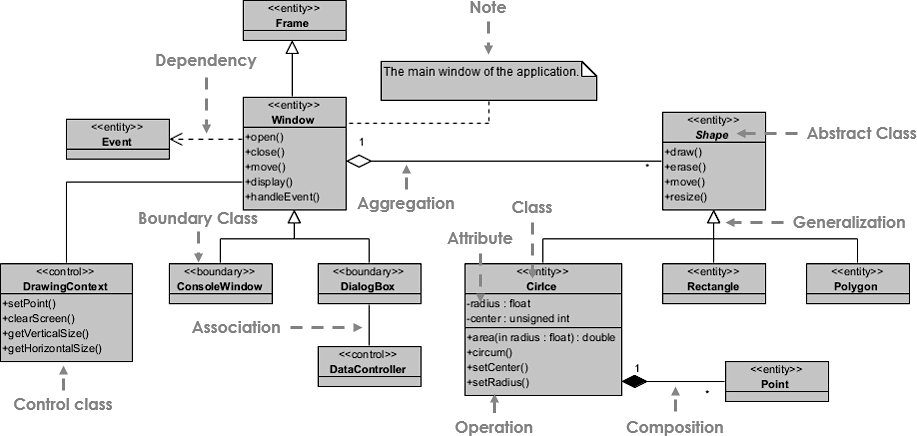
\includegraphics[width=\textwidth]{uml.png}
			\caption{GUI Class Diagram \cite{umlVisual}}
	\end{figure}

\section{OO Software Metrics}

\key{Control Flow Graphs}{Cyclomatic Complexity}{CK Metrics}

\defn{Metric}{quantitative measure of degree to which a
system, component or process possesses a given
attribute}

\defn{Indicator}{combination of metrics that provide insight into the
product/process}

\rem{metrics differs from measures in the sense that metrics are functions which
output measures~\cite{metricsWiki}}

\subsubsection{Motivation}

\begin{itemize}
	\item Budgeting 
	\item To create a baseline, in order to compare the impact of new tools
	\item Establish productivity trends and estimate staffing needs
	\item Improve software quality
\end{itemize}

\subsection{How can quality be measured?}

\par{In 1992 , Basili \cite{basili92} suggested a \ita{top-down} goal oriented
framework, to define what could me used as a measurement}

\begin{enumerate}
	\item Develop a set of goals
	\item Develop a set of questions which characterize those goals
	\item Specify the metrics required to answer 2
	\item Develop appropriate mechanisms for data collection and analysis
	\item Collect, validate and analyse the data
	\item Analyse in a \ita{post-mortem} fashion
	\item Provide feedback
\end{enumerate}

\subsubsection{Control Flow Graphs}

\defn{CFG}{a graph representing all possible paths that might be transverses
during the execution of a program} 

\par{We represent blocks of code as nodes in a graph, and draw edges between two
nodes \ita{iff} the execution of one of a node could transfer control to the one
being connected to it}

\par{In order to draw a CFG, we start by breaking the code into its major blocks
by identifying (1) Methods ; (2) Method Blocks ; (3) Decision Points . We then
translate this into nodes and connect them according to all possible execution states}

\ex{
\vphantom{.\\[2mm]}


\begin{minipage}{\linewidth}
      \centering
      \begin{minipage}{0.45\linewidth}
          \begin{figure}[H]
              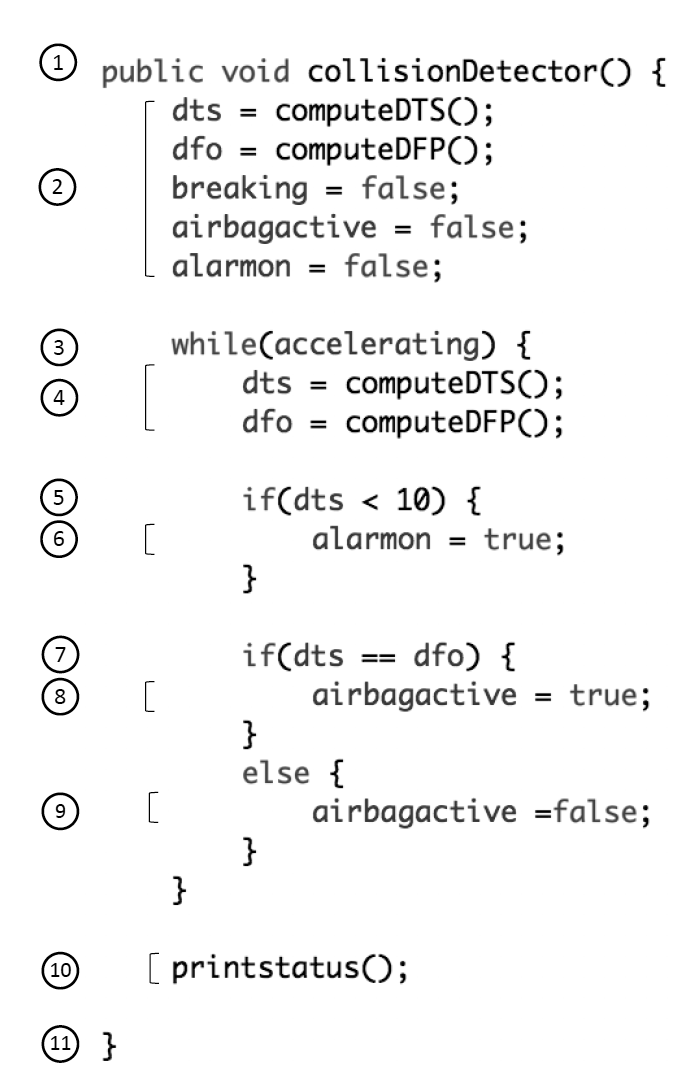
\includegraphics[width=\linewidth]{cfg}
          \end{figure}
      \end{minipage}
      \hspace{0.05\linewidth}
\begin{minipage}{0.45\linewidth}
          \begin{figure}[H]
              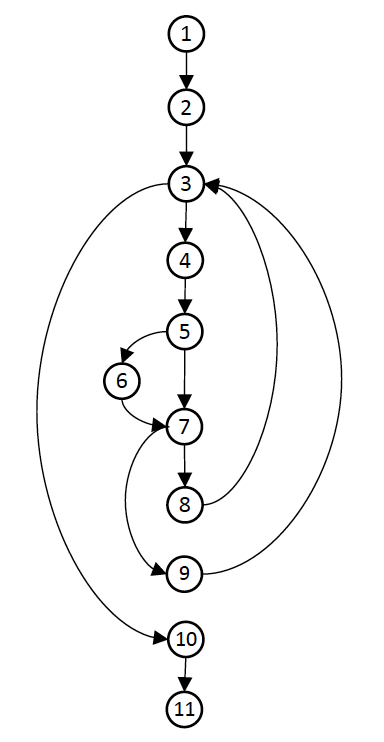
\includegraphics[width=\linewidth]{cfg2}
          \end{figure}
      \end{minipage}
\end{minipage}
}


\defn{Cyclomatic Number $V(G)$}{ of a graph $G$ on $n$ vertices and $e$ edges
with $p$ connected component. $V(G) = e - n + 2p$}

\par{Given the CFG, McCabe~\cite{mccabe76} introduced a graphic-theoretic
complexity measure and showed how it could be used to manage and control program
complexity. The goal was \ita{"to find a mathematical technique that
will provide a  quantitative basis for modularization and allow us to identify
software modules that will be difficult to test or maintain."} As a rule of
thumb, when restructuring code one aims to start with those with higher $V(G)$,
in order to lower their complexity}

\par{\mymarginpar{Pros \& Cons}~This is a fairly easy to compute metric, and
empirical studies have shown good correlation between cyclomatic complexity and
understandability. However, it is the hard to grasp the flow of data, and its
use might not be appropriate for OO programs.}

\subsection{CK Metrics}

\par{More recently, Chidamber and Kemerer \cite{chidamber_kemerer94}, introduced
6 other metrics, which are still in use today, despite the existence of $300+$
new ones}

\begin{enumerate}
	\item\textbf{WMC} : Weighted Methods per Class
	\item\textbf{DIT} : Depth of Inheritance Tree
	\item\textbf{NOC} : Number of Children
	\item\textbf{CBO} : Coupling Between Objects
	\item\textbf{RFC} : Response For a Class
	\item\textbf{LCOM} : Lack of Cohesion of Methods
\end{enumerate}

\par{A summary of the 6 metrics and how they affect complexity , re-usability
and modularity are presented below}

\begin{figure}[H]
	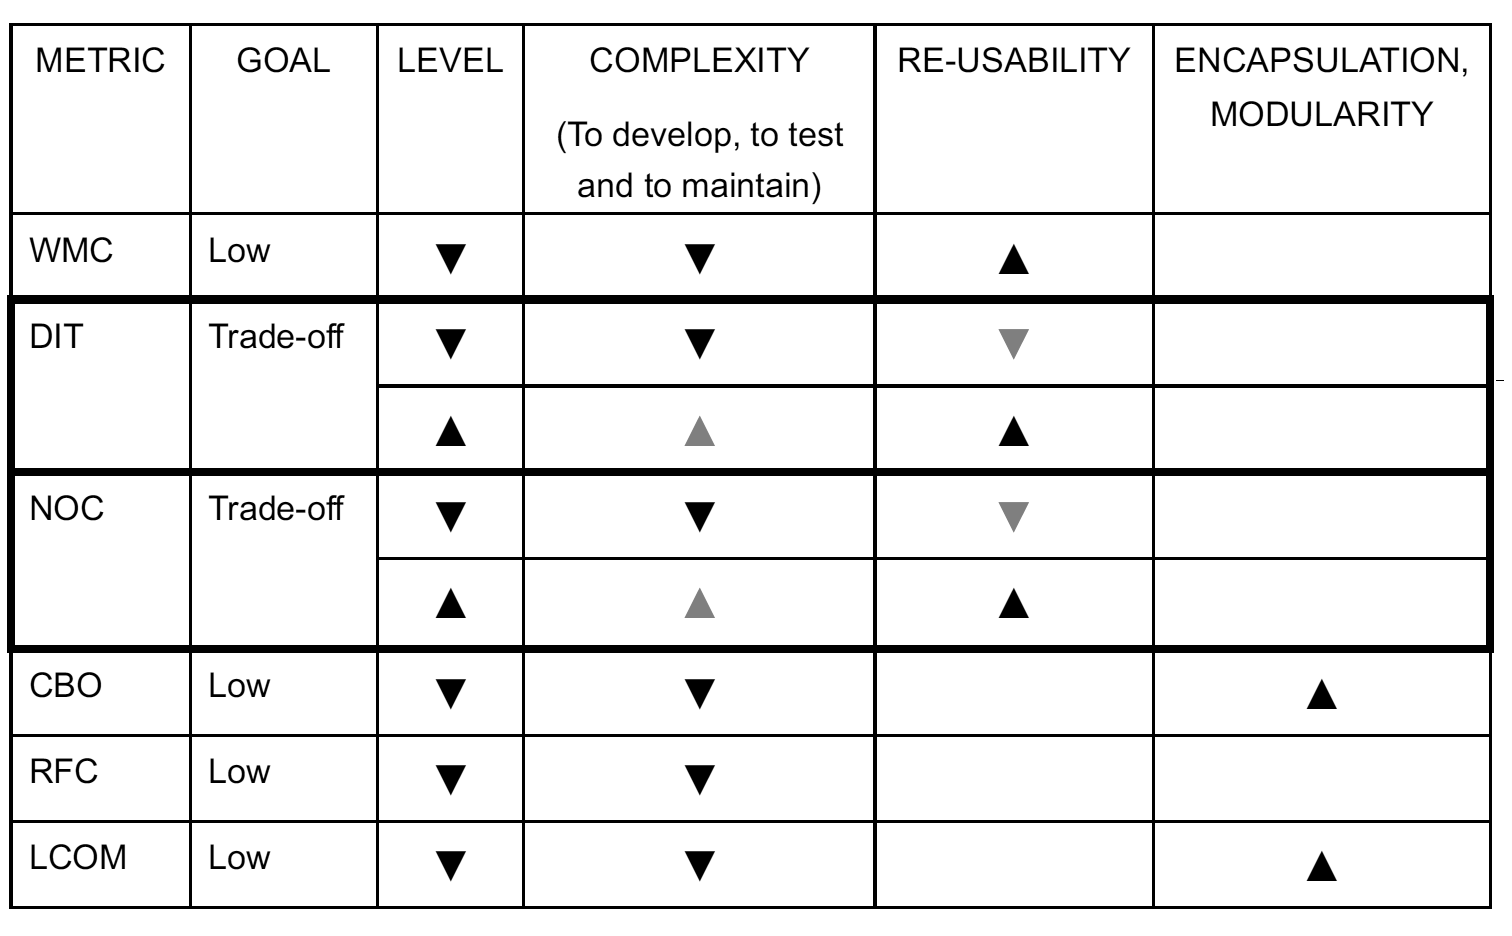
\includegraphics[width=\textwidth]{ck}
	\caption{CK Metrics : Summary}
\end{figure}

\par{Note that there exists a direct relation between the
metric level and complexity level, but sometimes one trades simplicity in favour
of reusability} 

\subsubsection{WMC}

$$\sum_{i=1}^{n}c_i$$

\par{WMC is the sum of the complexities of the methods in a given class, where
$c_i$ represents the McCabe complexity of each method. It acts as a predictor of
how much time and effort is required to develop and maintain that class}

\subsubsection{DIT}

\par{We define DIT as the length of any given node to the root of the tree.
Adding dependent methods, will increase complexity but improve reusability. The
goal is to achieve the appropriate trade-off for a given project}

\subsubsection{NOC}

\par{Similar to DIT, but we look at the number of \ita{direct} children only}

\subsubsection{CBO}

\par{For a given class $C$ , the CBO is the number of other classes to which $C$
is coupled to. Where we define classes to be "coupled" as "operating upon" or
"being operated on"}

\subsubsection{RFC}

\par{The number of methods of a class as well as any other methods being called
by methods within it}

\subsubsection{LCOM}

\par{Counts the sets of methods in a class that are not related
through the sharing of some of the class's fields. It measures the relative
\ita{"tightness"} of a class. The aim is to have as cohesive a class as
possible, otherwise we should wonder if two methods who share little to no
fields should belong to that same class. In practice, the lack of cohesion of a
class is calculated by subtracting the number of method pairs that don't share
access to the same fields by those who do}

\ex{
\vphantom{\\[2mm]}
	\lstinputlisting[language=C]{cohesion.c}
}

\section{Software Quality}

	\key{Static Analysis}{Bug
Patterns}{Soundness}{Precision}{Debugger}{Bug}{Debugging
Techniques}{Bytecode}{Source Code}{Bug Triage}{Software Reliability}

	\subsection{Introduction}

		\defn{Software Reliability}{denotes a product's trustworthiness or
dependability}

	\rem{software reliability varies \ita{directly} with the number of bugs}

		\defn{Bug}{a failure in a computer system that produces an incorrect or
unexpected result}

	\par{We can define a bug in terms of which outcome it produces given its
spec. In particular, we classify something as a bug, if one of the following
occurs}

		\begin{enumerate}\mymarginpar{$S$ is spec , $O$ is outcome, and $X$ is a
behaviour}
			\item $X \in S \land X \not\in O$
			\item $\neg X \in S \land X \in O$ 
			\item $X \not\in S \land X \in O$
			\item broken spec and broken outcome ; i.e. doesn't do X and it
isn't mentioned \ita{but it should}
			\item clunky software, broken from an untrained user's perspective 
		\end{enumerate}
	
		\subsubsection{Bug Causes}

		\par{The major cause of bugs occur at the specification level, followed
by the design stage and actual code}
		\par{At the spec level is often due to a breakdown in communication, or
a lack of formality in its implementation (e.g. not written, incomplete, sketch
only). The design stage is often overlooked or rushed, leading to
inappropriate modelling, or a lack of modeling tools. Coding errors can occur
due to a complex nature of the software, or simpler things like poor
documentation or limited time for project completion leading to rushed work}

	\rem{some coding codes examples are wrong messages, overflow errors,
override errors, misuse local variable, syntax ...}

	\rem{the cost of fixing a bug grows linearly with the life of a project,
from spec design to release}

	\subsection{Debugging Techniques}

	\defn{Bug Triaging}{is the assignment of a bug to the most
appropriate/capable developer who will fix it}

	\par{The triager needs to be aware of both the project, the bug reports and
the team involved in the project. A general workflow for bug is as follows:}

		\begin{enumerate}
			\item a bug is reported
			\item bug is assigned to manager for triage
			\item if fixed END , else assign to developer to fix
			\item re-test new code ; if fixed END else goto 2
		\end{enumerate}
 
	\defn{Static Analysis}{a method of a computer program debugging that is done
by examining the code without executing the program. It provides an
understanding of the code structure}

	\defn{Threat Modelling}{inspect at design stage, and draw out possible error
paths}
	
	\defn{Manual Code Reviews}{read source code, and reason based on your
knowledge whether bugs can occur}

	\rem{Note that this process can be quite subjective, depending on the
inspector}

	\defn{Automated Tools}{tools which parse program code, and automatically
detect common bugs}

	\rem{AT is particularly efficient for finding common bugs/bug patterns}

	\defn{Bug Pattern}{recurring correlations between signalled errors and
underlying bugs}

	\begin{enumerate}
		\item\textbf{Predictable random number generator} \par{given the
\ita{pseudo} nature of random generators, it is easy for a malicious user to get
hold of the next random number in a series. In Java, there's a better way to
generate random numbers by using the \texttt{SecureRandom} library instead of
the \texttt{Random}}
		\item\textbf{Object Deserialization} \par{object deserialization of
untrusted data can lead to remote code execution (e.g open attachments in
untrusted email sources).}
		\par{It is best to avoid untrusted sources, but when not possible, then
input validation is robustly applied for sanitation. Thus mitigating any
malicious input strings being converted to executable binary}

		\item\textbf{Trust Boundary Violation}\par{when the trust boundary is
blurred, and data is passed over the boundary without proper validation}
		\item\textbf{Null Pointer Exception}\par{when an object which does not
exist is accessed}
		\item\textbf{Infinite Recursion}a call to a recursive function that
never reaches the base case
	\end{enumerate}	

	\defn{Deserialization}{taking structured data (e.g JSON) and rebuild it into
an object} 

	\defn{Trust Boundary}{an imaginary line drawn through logical pieces of a
program where on one side we assume that the data is trustworthy, and on the other
untrustworthy}	

%%% COPY BUG CATEGORIES %%%

\par{Manually examine source code can be labour intensive and subjective
depending on the inspector}

	\defn{Debugger}{special program used to analyse other programs in order to
find bugs}

	\par{The debugger will analyse program code (e.g source, bytecode , etc) and
will analyse it in terms of the correctness of its statements, control flow,
method class , etc. without actually executing the code}
	
	\subsubsection{The Limitis of Static Analysis}
		
		\par{We can't really tell whether a program $P$ has some property $Q$ ,
instead we \ita{approximate} $Q$ in analysis $P$}	

	\rem{Recall \ita{Church-Turing's} introduction of the \ita{Halting
Problem}~\cite{turing1937}~\cite{church1936}}

	\defn{Soundness}{ if sound then an alert is
raised; unsound means that the detection system can generate false negatives
}

	\defn{Precision}{measures accuracy of bug detection. If precise then every
bug alert is an actual bug ; imprecise implies possible false positives}

	\par{Most analysis tools involve a trade-off between soundness, precision
and execution time. Though, the majority of tools are \ita{conservative} in
nature, i.e soundness is often preferred}

	\par{So, depending on the project, one can approximate towards:}
		\begin{itemize}
			\item\textbf{Completeness}\par{where the detection tool is
designed in a such a way so as to \ita{overestimate} possible program behaviours ;
with the drawback that the false positives might overshadow the real bugs}
			\item\textbf{Soundness}\par{where the detection tool
\ita{underestimates} the possible program behaviours ; with the drawback that the analysis is
incomplete}
		\end{itemize}

	\rem{in practice a \ita{balanced approximation}, which is neither sound nor
complete, allows for enough flexibility so that the program behaviour is more
easily estimated}
 



%%%%%%%%%%%%%%  BIBLIOGRAPHY  %%%%%%%%%%%%%%%%%%%
\newpage
\nocite{*}
\printbibliography

%%%%%%%%%%%%%%%%%%%%%%%%%%%%%%%%%%%%%%%%%%

\end{document}
